\chapter{Dual Ascent}\label{ch:dualascent}

The dual ascent algorithm is the dual version for the problem of the minimum
\emph{Steiner} tree, which tries to find a directed subtree that connects a
root node to a selected subset of existing nodes. If in the Steiner tree the
purpose is to minimize the total cost of the links used in the resulting
broadcast tree, in the dual ascent version the goal is to maximize a quantity
derived by the costs, named \emph{slack}. Both versions find the same lower
bound for the optimal solution, according to the mathematical definition of a
dual problem.

\section{Comparison with Dijkstra}\label{sec:comparison}

The Dijkstra algorithm tries to find a minimum \emph{spanning} tree which
contains links that connect a set of target nodes.

Differently from that, the minimum \emph{Steiner} tree considers for the
computations, to connect all the target nodes, also other nodes. So in this way
the lower bound of the optimal solution is less or equal than the result
provided by a \emph{spanning} tree algorithm (as we can see in
\figref{fig:steiner}). The price to pay is in term of time and computational
power, because the algorithm has to visit all the possible links and not the
subset that involves only the target nodes, so this solution has a limited
scalability.

\begin{figure}
	\centering
	\begin{subfigure}[b]{0.3\textwidth}
		\centering
		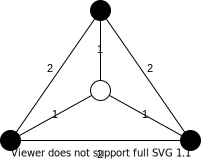
\includegraphics[width=\textwidth]{img/steiner-topology}
		\caption{An example of a network topology where black nodes are
		target nodes}\label{subfig:steiner-topology}
	\end{subfigure}
	\begin{subfigure}[b]{0.3\textwidth}
		\centering
		\includegraphics[width=\textwidth]{img/steiner-minspanning}
		\caption{The result of a minimum spanning tree algorithm on the
		example network topology. The result only contains links that
		involve target nodes. Its cost is
		4}\label{subfig:steiner-minspanning}
	\end{subfigure}
	\begin{subfigure}[b]{0.3\textwidth}
		\centering
		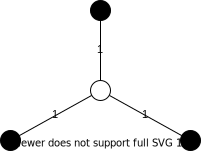
\includegraphics[width=\textwidth]{img/steiner-minsteiner}
		\caption{The result of a minimum Steiner tree algorithm on the
		example network topology. It includes also non-target nodes to
		build the tree. Its cost is 3}\label{subfig:steiner-minsteiner}
	\end{subfigure}
	\caption{An example of application of a minimum spanning tree algorithm
		and a minimum Steiner tree algorithm on the same
		topology}\label{fig:steiner}
\end{figure}


\section{The algorithm}\label{sec:algorithm}

The dual ascent algorithm starts from the source (root) node and works
iteratively. There are three important data structures:

\begin{description}
	\item[Root Component] A set of strongly connected nodes, containing at
		least a target one, which hasn't incoming links from other
		target nodes or from the root node.
	\item[Auxiliary Graph] A graph which starts with all the topology nodes
		(including the non-target ones) and no links. At each iteration
		of the algorithm, the link with the minimum cost is added.
	\item[Reduced Cost Table] A table which stores the
		costs of connected nodes. Element \(R_{ij}\) represents the cost
		from the node \(i\) to reach the node \(j\). The final
		cost of the algorithm is the sum of all \(R_{kk}\) values
		(slacks), where \(k\) is the index of a target node.
\end{description}

At each step a list of current root components is extracted from the auxiliary
graph. For each element of the list the algorithm finds, from the starting
topology, the link with minimum cost that has the root component as destination
and adds it to the auxiliary graph. Then the reduced cost table is updated by
decreasing the new cost value with the one that involved that nodes, selected at
the first iteration of the algorithm (the minimum one). The value obtained is
the \emph{slack}, quantity to maximize as the purpose of the algorithm, that is
memorized into \(R_{jj}\) elements. Also values \(R_{ij}\) are updated
considering the new paths formed in the auxiliary graph.

These steps are done until there are no remaining root components or no new
links from the starting topology. If in the auxiliary graph there are any
cycles, they are resolved deleting highest cost paths, so that the final result
is a broadcast tree including all the target nodes with zero or some non-target
ones.

